\mySection{10.3 Goodness-of-Fit Tests: All Parameters Known}
%-------------- start slide -------------------------------%{{{ 10.16
\begin{frame}
	% {\S\: 10.3 Goodness-of-Fit Tests: All Parameters Known}
	\begin{enumerate}
		\item[Rationale]
		\item[$!$] We want to test if the c.d.f. $F_Y(\cdot)$ is given by the true c.d.f. $F_0(\cdot)$, i.e., \\[1em]
			\[H_0:F_Y(y) = F_0(y)\quad v.s. \quad H_1: F_Y(y)\ne F_0(y)
			\]
			\vfill
		\item[$\sim$] By properly partitioning the domain, the random sample should follow
		\begin{center}
			\textcolor{yellow!80!black}{\it an induced multinomial distribution}.
		\end{center}
		\vfill
		\item[$\Longrightarrow$] Then testing $F_Y(\cdot)=F_0(\cdot)$ reduces to testing the induced multinomial distribution of the following form: \\[1em]
			\[
			H_0: p_1 = p_1', \cdots, p_n =p_n'
			\]
			\[
			v.s.
			\]
			\[
				H_1: p_i\ne p_i'\quad\text{for at least one $i$}
			\]
	\end{enumerate}
\end{frame}
%-------------- end slide -------------------------------%}}}
%-------------- start slide -------------------------------%{{{ 10.17
\begin{frame}[fragile]

	\begin{enumerate}
		\item[How]
		\item Suppose we are sampling from the c.d.f. $F(y)$
			\vfill
		\item Divide the range of the distribution into $k$ mutually exclusive and exhausive intervals, say $I_1,\cdots, I_k$.
			\vfill
		\item Let $\pi_i = \bbP(X\in I_i)$, $i=1,\cdots, k$.
			\vfill
		\item Let $O_1,\cdots,O_k$ be the respective
			observed numbers of the observations $X_1,\cdots, X_n$ in
			the intervals $I_1,\cdots,I_k$.
			\vfill
		\item Then $O=(O_1,\cdots,O_k)\sim $ multinomial distribution with $(\pi_1,\cdots,\pi_k)$, i.e.,
			\[
				\bbP\left(O_1=o_1,\cdots, O_k=o_k \right )
				=\frac{n!}{\prod_{i=1}^k o_i!}\prod_{i=1}^k \pi_i^{o_i}
			\]
			with  $\sum_{i=1}^k \pi_i=1$, $\sum_{i=1}^k o_i = n$, and
			\[
				\E[O_i] = n\pi_i =:e_i, \quad \Var(O_i) = n \pi_i(1-\pi_i)
			\]
	\end{enumerate}
\end{frame}
%-------------- end slide -------------------------------%}}}
%-------------- start slide -------------------------------%{{{ 10.18
\begin{frame}[fragile]

	\begin{enumerate}
		\setcounter{enumi}{5}
		\item When $k=2$, by CLT,  as $n\rightarrow \infty$,
			\[
				\frac{O_1-n\pi_1}{\sqrt{n\pi_1(1-\pi_1)}}\stackrel{d}{\rightarrow} N(0,1)\quad
				\Longrightarrow\quad
				\frac{(O_1-n\pi_1)^2}{n\pi_1(1-\pi_1)}\stackrel{d}{\rightarrow}\chi^2_1
			\]
		\item[]
				\[\hspace{12em}||\]
			\[
\hspace{12em}\frac{(O_1-n\pi_1)^2}{n\pi_1}
+\frac{(O_2-n\pi_2)^2}{n\pi_2}
			\]
		\item[]
			\[\hspace{12em}||\]
			\[
				\hspace{12em}\frac{(O_1-e_1)^2}{e_1}
				+\frac{(O_2-e_2)^2}{e_2}
			\]
			\vfill
		\item[] Hence, as $n\to\infty$,
			\[
				\sum_{i=1}^k
				\frac{(O_i-e_i)^2}{e_i}\stackrel{d}{\rightarrow}\chi^2_{k-1}
			\]
	\end{enumerate}
\end{frame}
%-------------- end slide -------------------------------%}}}
%-------------- start slide -------------------------------%{{{ 10.19
\begin{frame}[fragile]

	\begin{enumerate}
		\setcounter{enumi}{6}
\item For general $k$,
			\[
\sum_{i=1}^k
\frac{(O_i-n\pi_i)^2}{n\pi_i} =
\sum_{i=1}^k
\frac{(O_i-e_i)^2}{e_i}
			\]
			follows a complicated, but exact, distribution, from which, one can show
			\[
	\sum_{i=1}^k
\frac{(O_i-e_i)^2}{e_i} \stackrel{d}{\rightarrow}\chi^2_{k-1}
			\]
			\vfill
		\item[]
			\[\Downarrow\]
			\vfill
		\item[Thm.] When $n$ is large enough, namely, when $n\pi_i\ge 5$ for all $i$,
			\[
				D=	\sum_{i=1}^k
				\frac{(O_i-e_i)^2}{e_i} \stackrel{appr.}{\sim}\chi^2_{k-1}.
			\]
			\vfill
		\item[Rmk:] The above is called {\em Pearson's chi-square test}. It is asymptotically equivalent to the generalized likelihood ratio test.
	\end{enumerate}
\end{frame}
%-------------- end slide -------------------------------%}}}
%-------------- start slide -------------------------------%{{{ 10.20
\begin{frame}[fragile]{Alternative: G-test\\
	\small -- the likelihood ration test for multinomial model}

	\begin{enumerate}
		\item Under $H_0:\pi_i=p_i$, $i=1,\cdots,k$, the MLE of $\pi_i$ are
			\[
				\widetilde\pi_i = p_i =  \frac{np_i}{n} =  \frac{e_i}{n},\qquad \forall i.
			\]
			\vfill
		\item When there are no constraints, for $i=1,\cdots,k-1$,
			\[
				\frac{\partial}{\partial \pi_i} \ln L(\pi_1,\cdots,\pi_{k-1}|o_1,\cdots,o_k)  = 0  ,\quad 1\le i\le k-1
			\]
			\[\text{\rotatebox[origin=c]{90}{$\Leftrightarrow$}}\]
			\[
				\frac{o_i}{\widehat\pi_i} = \frac{o_k}{1-\widehat\pi_1-\cdots - \widehat\pi_{k-1}},\quad 1\le i\le k-1
			\]
			\[\text{\rotatebox[origin=c]{90}{$\Leftrightarrow$}}\]
			\[
				\widehat\pi_i = \frac{o_i}{n},\quad 1\le i\le k.
			\]
	\end{enumerate}
\end{frame}
%-------------- end slide -------------------------------%}}}
%-------------- start slide -------------------------------%{{{ 10.21
\begin{frame}[fragile]

	\begin{enumerate}
		\setcounter{enumi}{3}
	\item[$\Rightarrow$]
		\begin{align*}
			\lambda := \ln \left( \frac{L(\widetilde\pi_1,\cdots,\widetilde\pi_{k-1}|o_1,\cdots,o_k)}{L(\widehat\pi_1,\cdots,\widehat\pi_{k-1}|o_1,\cdots,o_k)} \right)
			&= \log \left( \frac{\prod_{i=1}^k \widetilde{\pi}_i^{o_i}}{\prod_{i=1}^k \widehat{\pi}_i^{o_i}}\right)\\
			\\&=\sum_{i=1}^k o_i \ln \left(  \frac{\widetilde\pi_i}{\widehat\pi_i}\right )
			\\&=\sum_{i=1}^k o_i \ln \left(  \frac{e_i}{o_i}\right )
		\end{align*}
	\item[] Critical region: $\lambda<\lambda_*<0$.
		\vfill
	\item[Def.]
		\[
			G: = -2 \lambda = -2\sum_{i=1}^k o_i \ln \left(  \frac{e_i}{o_i}\right )
=2\sum_{i=1}^k o_i \ln \left(  \frac{o_i}{e_i}\right )
		\]
	\item[] $G \stackrel{approx.}{\sim} \chi^2_{k-1}$ for large $n$.
	\item[] Critical region: $G\ge G_* = \chi^2_{1-\alpha,k-1}$.
\end{enumerate}
\end{frame}
%-------------- end slide -------------------------------%}}}
%-------------- start slide -------------------------------%{{{ 10.22
\begin{frame}[fragile]

	\begin{enumerate}
		\item[Relation] G-test and Pearson's Chi square test
			\vfill
		\item[] By second order Taylor expanson around $1$,
			\begin{align*}
				G &= -2 \sum_{i=1}^k o_i \ln \left(  \frac{e_i}{o_i}\right )\\
				  &\approx
				  -2\sum_{i=1}^k o_i \left[ \left( \frac{e_i}{o_i} -1\right )-\frac12 \left(\frac{e_i}{o_i}-1 \right )^2  \right ]
				\\&=
				-2\sum_{i=1}^k (e_i-o_i) + \sum_{i=1}^k o_i\left(\left(1-\frac{o_i}{e_i}\right)+\frac{o_i}{e_i} \right)\left(\frac{e_i}{o_i}-1 \right )^2
				\\& = 0 + \sum_{i=1}^n \frac{o_i^2}{e_i} \left(1-\frac{o_i}{e_i} \right)^3 +  \sum_{i=1}^k \frac{(e_i-o_i)^2}{e_i}
				\\& \approx \sum_{i=1}^k \frac{(e_i-o_i)^2}{e_i}
			\end{align*}
		\item[]
			\vspace{-1em}
			\begin{minipage}{0.5\textwidth}
			\[||\]
			\[D\]
			\end{minipage}
			\vfill
		\item[$\therefore$] Pearson's Chi-square test is an approximation of G-test.
	\end{enumerate}
\end{frame}
%-------------- end slide -------------------------------%}}}
%-------------- start slide -------------------------------%{{{ 10.23
\begin{frame}
\begin{enumerate}
\item[E.g. 1] {\it Benford's law}:
\begin{center}
\begin{minipage}{0.5\textwidth}
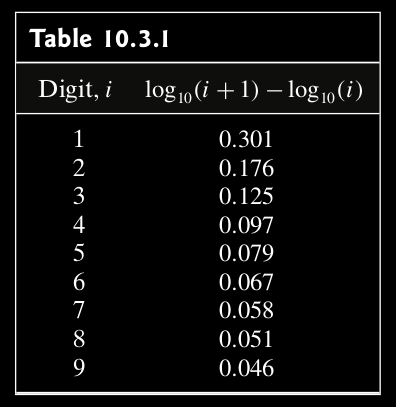
\includegraphics[scale=0.3]{Table_10-3-1-neg.png}
\end{minipage}
% \hspace{2em}
\begin{minipage}{0.333\textwidth}
Initial digits\\
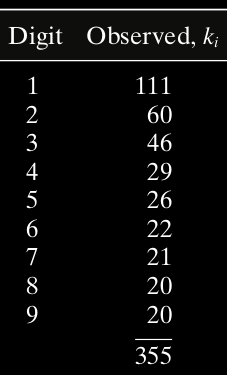
\includegraphics[scale=0.25]{Table_10-3-2-2-neg.png}
\end{minipage}
\end{center}
Use this law to check whether the bookkeepers have made up entries. \\[1em]
Assume that bookkeepers are not aware of Benford's law.
\end{enumerate}
\end{frame}
%-------------- end slide -------------------------------%}}}
%-------------- start slide -------------------------------%{{{ 10.24
\begin{frame}

\begin{enumerate}
\item[Sol.] The test should be
\begin{align*}
&H_0: p_1=p_{10},\cdots,p_9=p_{90}
\\& \hspace{4em} v.s.\\ &
H_1: p_i\ne p_{i0} \quad \text{for at least one $i=1,\cdots, 9$.}
\end{align*}
% \item[]
% \begin{center}
% 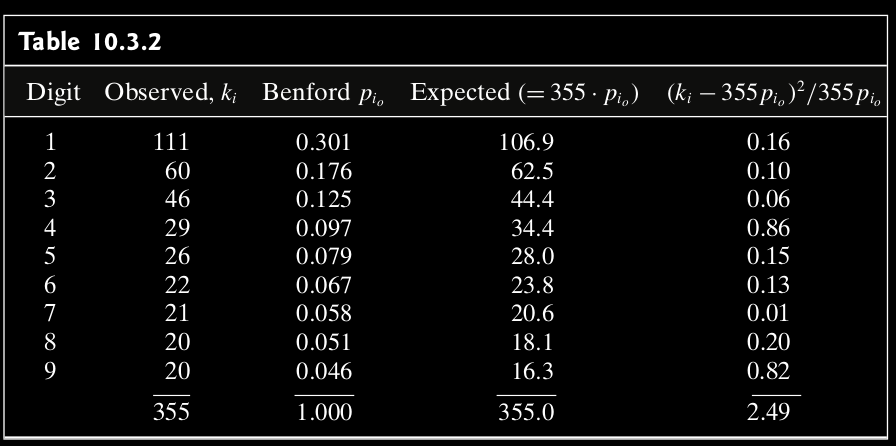
\includegraphics[scale=0.3]{Table_10-3-2-neg.png}
% \end{center}
\vfill
\item[] Critical region: $\left(\chi_{.95,8}^2,\infty \right)=(15.507,\infty)$.
\end{enumerate}
\end{frame}
%-------------- end slide -------------------------------%}}}
%-------------- start slide -------------------------------%{{{ 10.25
\begin{frame}[fragile]
		Compute the $D$ and $G$ scores:
		\vfill
			\begin{center}
				 \renewcommand{\arraystretch}{1.6}
				\begin{tabular}{ccc|ccc}
					\hline
			Digit & $o_i$ & $p_i$ & $e_i$ & $(o_i-e_i)^2/e_i$              & $2o_i\ln(e_i/o_i)$ \\ \hline
			1     & 111   & 0.301 &       &                                & \cr
			2     & 60    & 0.176 &       &                                & \cr
			3     & 46    & 0.125 &       &                                & \cr
			4     & 29    & 0.097 &       &                                & \cr
			5     & 26    & 0.079 &       &                                & \cr
			6     & 22    & 0.067 &       &                                & \cr
			7     & 21    & 0.058 &       &                                & \cr
			8     & 20    & 0.051 &       &                                & \cr
			9     & 20    & 0.046 &       &                                & \cr \hline
			sum   & 355   & 1     & 355   & $d=\underline{\phantom{aaaa}}$ & $g=\underline{\phantom{aaaa}}$ \cr \hline
	\end{tabular}
	\end{center}
\end{frame}
%-------------- end slide -------------------------------%}}}
%-------------- start slide -------------------------------%{{{ 10.26
\begin{frame}[fragile]
	\begin{center}
	\renewcommand{\arraystretch}{1.6}
		\begin{tabular}{ccc|ccc}
			\hline
			Digit & $o_i$ & $p_i$ & $e_i$ & $(o_i-e_i)^2/e_i$    & $2o_i\ln(e_i/o_i)$ \\ \hline
			1     & 111   & 0.301 & 106.9 & 0.16                 & 8.449\cr
			2     & 60    & 0.176 & 62.5  & 0.10                 & -4.860\cr
			3     & 46    & 0.125 & 44.4  & 0.06                 & 3.309\cr
			4     & 29    & 0.097 & 34.4  & 0.86                 & -9.963\cr
			5     & 26    & 0.079 & 28.0  & 0.15                 & -3.937\cr
			6     & 22    & 0.067 & 23.8  & 0.13                 & -3.433\cr
			7     & 21    & 0.058 & 20.6  & 0.01                 & 0.828\cr
			8     & 20    & 0.051 & 18.1  & 0.20                 & 3.982\cr
			9     & 20    & 0.046 & 16.3  & 0.82                 & 8.109\cr \hline
			sum   & 355   & 1     & 355   & $d=\underline{2.49}$ & $g=\underline{2.48}$\cr\hline
		\end{tabular}
	\vfill
	Conclusion: Fail to reject.
	\end{center}
\end{frame}
%-------------- end slide -------------------------------%}}}
%-------------- start slide -------------------------------%{{{ 10.27
\begin{frame}[fragile]
	\begin{center}
	\begin{lstlisting}
> #  EX 10.3.2
> library(data.table)
> mydat <- fread('http://math.emory.edu/~lchen41/teaching/2020_Spring/Case_10-3-2.data')
trying URL 'http://math.emory.edu/~lchen41/teaching/2020_Spring/Case_10-3-2.data'
Content type 'unknown' length 153 bytes
==================================================
downloaded 153 bytes

> head(mydat)
   Digit  Oi    Pi
1:     1 111 0.301
2:     2  60 0.176
3:     3  46 0.125
4:     4  29 0.097
> pi = mydat[,3]
> oi = mydat[,2]
> n = sum(oi)
> ei = n*pi
> di = (ei-oi)^2/ei
> gi =  2*oi*log(oi/ei)
> print(paste("Using Pearson's test, D value is equal to ", round(sum(di),3)))
[1] "Using Pearson's test, D value is equal to  2.491"
> print(paste("Using the G-test, G value is equal to ", round(sum(gi),3)))
[1] "Using the G-test, G value is equal to  2.484"
	\end{lstlisting}
\footnotesize
Codes available
\\
\baseurl{Case_10-3-2.R}
	\end{center}
\end{frame}
%-------------- end slide -------------------------------%}}}
%-------------- start slide -------------------------------%{{{ 10.28
\begin{frame}
\begin{enumerate}
\item[E.g. 2] Test for randomness\\[1em]
Is the following sample of size $40$ from $f_Y(y)=6y(1-y)$, $y\in[0,1]$?
\vfill
\begin{center}
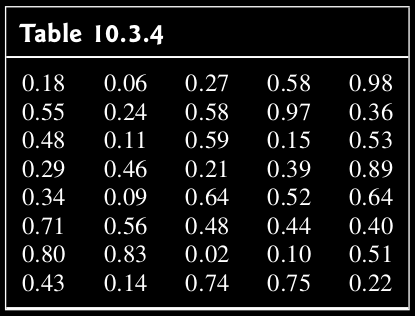
\includegraphics[scale=0.3]{Table_10-3-4-neg.png}
\end{center}
\end{enumerate}
\end{frame}
%-------------- end slide -------------------------------%}}}
%-------------- start slide -------------------------------%{{{ 10.29
\begin{frame}

\begin{enumerate}
\item[Sol.] Test continuous pdf $\rightarrow$ reduce to a set of classes:
\begin{center}
% 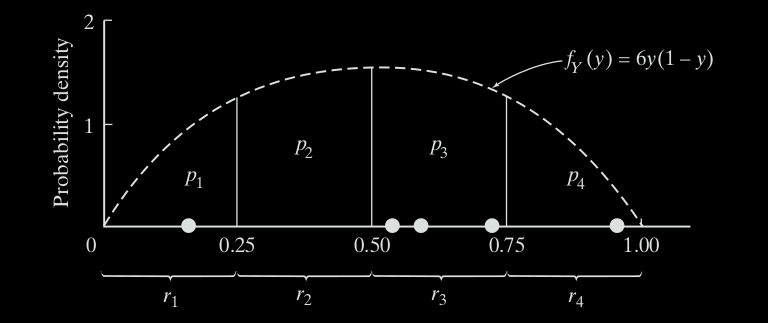
\includegraphics[scale=0.18]{Figure_10-2-2-neg.png}	\\ \pause
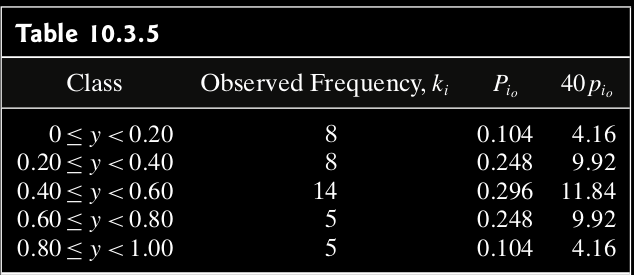
\includegraphics[scale=0.25]{Table_10-3-5-neg.png}\\ \pause
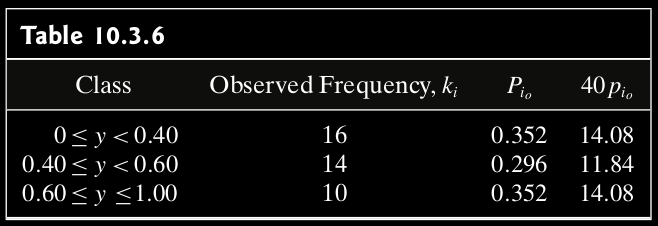
\includegraphics[scale=0.24444]{Table_10-3-6-neg.png} \pause
\end{center}
\[
d = \cdots =1.84.
\]
\item[] Critical region: $\left(\chi_{.95,2}^2,\infty \right)=(5.992,\infty)$.
\item[] Conclusion: Fail to reject.
\end{enumerate}
\end{frame}
%-------------- end slide -------------------------------%}}}
%-------------- start slide -------------------------------%{{{ 10.30
\begin{frame}[fragile]
	\begin{lstlisting}
> # Case Study 10.3.2
> # Read data from the URL link
> library(data.table)
> mydat <- fread('http://math.emory.edu/~lchen41/teaching/2020_Spring/EX_10-3-1.data')
trying URL 'http://math.emory.edu/~lchen41/teaching/2020_Spring/EX_10-3-1.data'
Content type 'unknown' length 234 bytes
==================================================
downloaded 234 bytes

>d(mydat)
   Col1 Col2 Col3 Col4 Col5
   1: 0.18 0.06 0.27 0.58 0.98
   2: 0.55 0.24 0.58 0.97 0.36
   3: 0.48 0.11 0.59 0.15 0.53
   4: 0.29 0.46 0.21 0.39 0.89
   5: 0.34 0.09 0.64 0.52 0.64
   6: 0.71 0.56 0.48 0.44 0.40
# Conditions for lower bounds
> lb=c(0,0.40,0.60)
> # Conditions for upper bounds
> up=c(0.40,0.60,1.00)
> # Store the results in d
> oi <- seq(1:length(lb))
> pi <- seq(1:length(lb))
> integrand <- function(y) {6*y*(1-y)}
> for (i in c(1:length(lb))) {
+   oi[i] <- table(mydat>=lb[i] & mydat<up[i])[2]
+   pi[i] <- integrate(integrand,  lb[i], up[i])$value[1]
+   print(paste("the", i,"th bin has", oi[i],
+       "entries and pi is equal to", pi[i]))
+ }
	\end{lstlisting}
\end{frame}
%-------------- end slide -------------------------------%}}}
%-------------- start slide -------------------------------%{{{ 10.31
\begin{frame}[fragile]
\begin{center}
\begin{minipage}{0.8\textwidth}
\begin{lstlisting}
[1] "the 1 th bin has 16 entries and pi is equal to 0.352"
[1] "the 2 th bin has 14 entries and pi is equal to 0.296"
[1] "the 3 th bin has 10 entries and pi is equal to 0.352"
> pi <- unlist(pi)
> n <- sum(oi)
> ei <- n*pi
> di <- (ei-oi)^2/ei
> gi <-  2*oi*log(oi/ei)
> rbind(oi,pi,ei,di,gi)
         [,1]       [,2]      [,3]
oi 16.0000000 14.0000000 10.000000
pi  0.3520000  0.2960000  0.352000
ei 14.0800000 11.8400000 14.080000
di  0.2618182  0.3940541  1.182273
gi  4.0906679  4.6920636 -6.843405
> print(paste("Using Pearson's test, D value is equal to ",round(sum(di),3)))
[1] "Using Pearson's test, D value is equal to  1.838"
> print(paste("Using the G-test, G value is equal to ", round(sum(gi),3)))
[1] "Using the G-test, G value is equal to  1.939"<Paste>
\end{lstlisting}
\end{minipage}
\vfill
\baseurl{EX_10-3-1.R}
\end{center}
\end{frame}
%-------------- end slide -------------------------------%}}}
%-------------- start slide -------------------------------%{{{ 10.32
\begin{frame}

\begin{enumerate}
\item[E.g. 3] Fisher's suspicion on Mendel's experiments on 1866:
\\
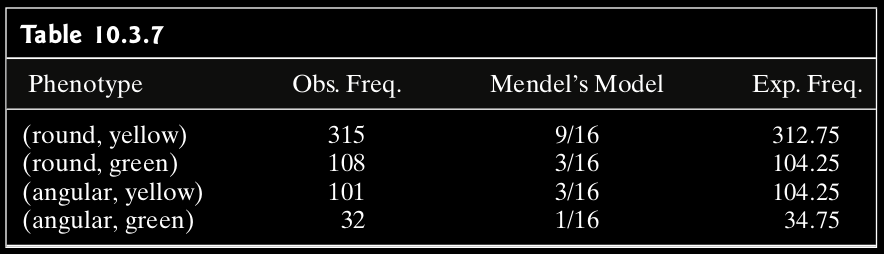
\includegraphics[scale=0.3]{Table_10-3-7-neg.png}
\vfill
\[
d= ... = 0.47
\]
\vfill
\[
P\text{-value} = \bbP(\chi_{3}^2 \le 0.47) = 0.0746.
\]
\end{enumerate}
\end{frame}
%-------------- end slide -------------------------------%}}}
%-------------- start slide -------------------------------%{{{ 10.33
\begin{frame}[fragile]

\begin{minipage}{0.4\textwidth}
\centering
\begin{lstlisting}
> # Case Study 10.3.3
> x=seq(0,10,0.1)
> plot(x,dchisq(x,3),type = "l")
> abline(v=0.47,col = "gray60")
> text(0.47,0,"0.47")
> title("Chi Square distribution
+       of freedom 3")
> pchisq(0.47,3)
[1] 0.07456892
\end{lstlisting}
\end{minipage}
\hfill
\begin{minipage}{0.5\textwidth}
\centering
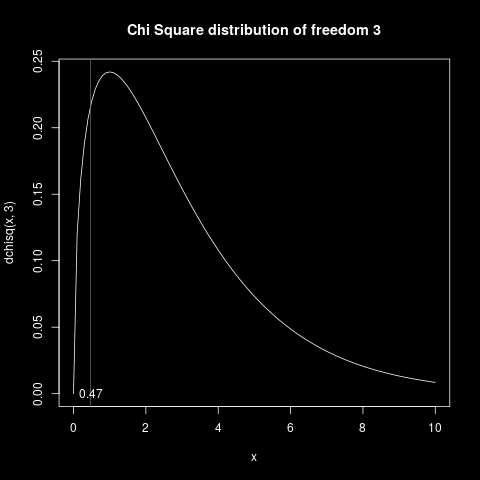
\includegraphics[scale=0.35]{Figure_10-3-4-neg.png}
\end{minipage}

\end{frame}
%-------------- end slide -------------------------------%}}}
%-------------- start slide -------------------------------%{{{ 10.34
\begin{frame}[fragile]

\begin{enumerate}
	\item[E.g. 2'] A second look at the random generator in E.g. 2.\\[1em]
		Does it fit the model too well? Find the $P$-value. \\
\vfill
\begin{minipage}{0.4\textwidth}
\centering
\begin{lstlisting}
> # Example 10.3.1
> x=seq(0,10,0.1)
> plot(x,dchisq(x,2),type = "l")
> abline(v=1.84,col = "gray60")
> text(1.84,0,"1.84")
> title("Chi Square distribution
+       of freedom 2")
> pchisq(1.84,2)
[1] 0.601481
\end{lstlisting}
\end{minipage}
\hfill
\begin{minipage}{0.5\textwidth}
\centering
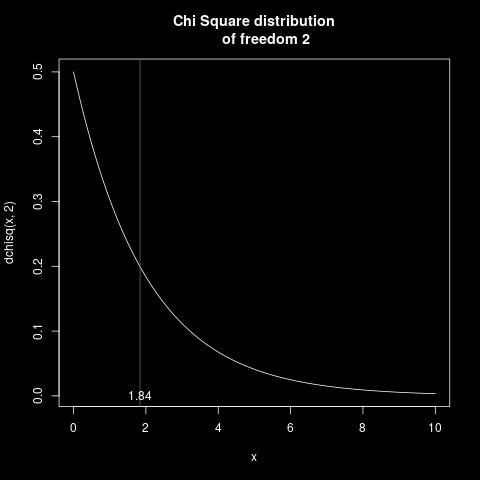
\includegraphics[scale=0.35]{Figure_Example-10-3-1-neg.png}
\end{minipage}
\vfill
\[
	P\text{-value} = 0.601\quad\Longrightarrow \quad \text{No.}
\]
\end{enumerate}
\end{frame}
%-------------- end slide -------------------------------%}}}
